Um die Funktion des Lock-In-Verstärkers kennenzulernen stehen ein modular
aufgebauter Verstärker(Abbildung \ref{fig:verstärker}) und ein
Speicher-Oszilloskop zur Verfügung.
\begin{figure}[h]
  \centering
  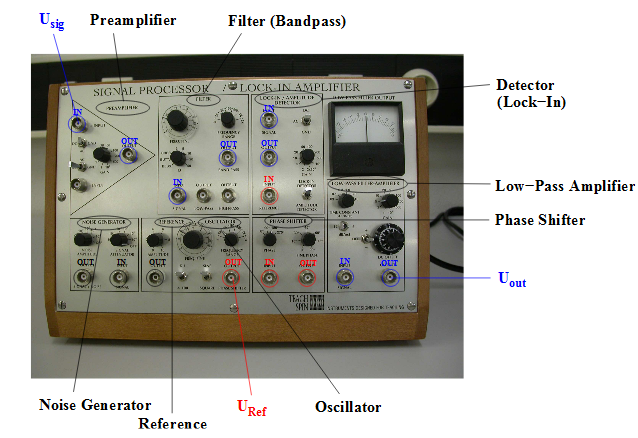
\includegraphics[width=\textwidth]{Bilder/Verstaerker.jpeg}
  \caption{Verstärker}
  \label{fig:verstärker}
\end{figure}
\\
Ein Lock-In-Verstärker besteht in der Regel aus folgenden Bauteilen:
\begin{itemize}
  \item Vorverstärker
  \item Hoch-, Tief- und Bandpassfilter
  \item Phasenverschieber für die Anpassung zwischen Referenz- und Messignal
  \item Funktionsgenerator
  \item Rauschgenerator
  \item Tiefpass-Verstärker
  \item Amplituden/Lock-In-Detektor
\end{itemize}
Die Signale der einzelnen Komponenten können über das verwendete
Speicher-Oszilloskop seperat betrachtet und vermessen werden.
In einem ersten Schritt wird die Schaltung aus der Abbildung \ref{fig:schalt}
aufgebaut.
\begin{figure}[h]
  \centering
  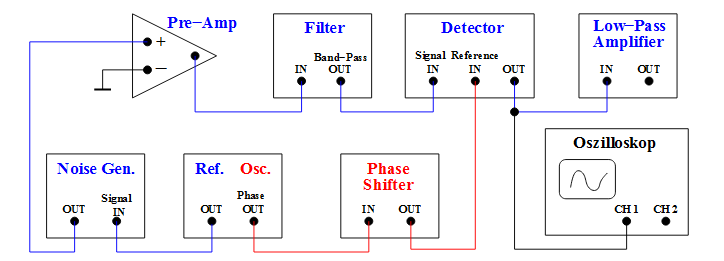
\includegraphics[width=\textwidth]{Bilder/Schaltung.jpeg}
  \caption{Schaltbild Lock-In-Verstärker}
  \label{fig:schalt}
\end{figure}
\\
Hierbei wird nach jedem Bauteil überprüft, welche Signalformen ausgegeben werden.
